\documentclass{article}
% For anonymous submission (NeurIPS review):
\usepackage[preprint]{neurips_2026}
% For preprint / arXiv (shows authors):
% \usepackage[preprint]{neurips_2026}
\usepackage[utf8]{inputenc}
\usepackage[T1]{fontenc}
\usepackage{hyperref}
\usepackage{url}
\usepackage{booktabs}
\usepackage{amsfonts}
\usepackage{amsmath}
\usepackage{amssymb}
\usepackage{amsthm}
\usepackage{graphicx}
\usepackage{xcolor}
\usepackage{subcaption}

\newtheorem{theorem}{Theorem}
\newtheorem{lemma}[theorem]{Lemma}
\newtheorem{corollary}[theorem]{Corollary}
\newtheorem{definition}[theorem]{Definition}
\newtheorem{proposition}[theorem]{Proposition}
\newtheorem{remark}[theorem]{Remark}
\newtheorem{axiom}{Axiom}

\newcommand{\R}{\mathbb{R}}
\newcommand{\E}{\mathbb{E}}
\newcommand{\Var}{\mathrm{Var}}
\newcommand{\SHAP}{\mathrm{SHAP}}
\newcommand{\DASH}{\textsc{Dash}}
\newcommand{\GBDT}{\textsc{GBDT}}

\title{The Attribution Impossibility}

% Author block hidden for anonymous review.
% Uncomment for camera-ready / arXiv preprint:
\author{
  Drake Caraker\thanks{Corresponding author: \texttt{drakecaraker@gmail.com}} \quad
  Bryan Arnold\thanks{\texttt{puremath86@gmail.com}} \quad
  David Rhoads\thanks{\texttt{drhoads9@gmail.com}} \\[4pt]
  \textit{Independent Researchers}
}

\begin{document}

\maketitle

\begin{abstract}
No feature ranking can be simultaneously faithful, stable, and complete when features are correlated. For collinear pairs, the ranking is literally a coin flip: retraining with a different seed inverts the importance ordering 50\% of the time.
Faithful, stable, and complete feature rankings cannot coexist under collinearity---we characterize the complete design space: exactly two families of methods exist, and no method lies outside this dichotomy.
The impossibility is quantitative: we derive architecture-discriminating bounds showing the attribution ratio diverges as $1/(1{-}\rho^2)$ for gradient boosting, is infinite for Lasso, and converges for random forests.
\DASH{} (\textbf{D}iversified \textbf{A}ggregation of \textbf{SH}AP) ensemble averaging is provably Pareto-optimal on the stable branch, achieving the Cram\'er--Rao variance bound with a tight ensemble size formula.
In a survey of 77 public datasets, 68\% exhibit attribution instability (conservative lower bound: survey power 32\% at the 10\% threshold; true prevalence likely higher).
Switching to conditional SHAP does not escape the impossibility when features have equal causal effects.
The framework includes practical diagnostics---a $Z$-test workflow and single-model screening tool---and has direct consequences for fairness auditing.
SHAP-based proxy discrimination audits are provably no better than coin flips under collinearity.
The design space theorem, diagnostics, and impossibility are mechanically verified in Lean~4 (305 theorems from 14 domain-specific + 2 query-complexity axioms, 0 \texttt{sorry})---to our knowledge, the first formally verified impossibility in explainable AI.
\end{abstract}

\section{Introduction}
\label{sec:intro}

Train a gradient-boosted model on your data. Compute SHAP values. Retrain with a different random seed. The `most important feature' changes. In a survey of 77 public datasets, 68\% exhibit this instability. Most practitioners assume this is an engineering problem---insufficient data, poor hyperparameters, or a software bug. We prove it is none of these. It is a mathematical impossibility.

Before this work, practitioners attributed SHAP instability to fixable causes. After, they know it is a mathematical certainty under collinearity---and they have a provably optimal fix.

\paragraph{A concrete example.}
Consider a credit model with annual income and debt-to-income ratio ($|\rho| = 0.72$): across 20 retrains, SHAP reports income as the top driver 53\% of the time and DTI 47\%, so a compliance report citing ``income'' as the primary adverse factor is a coin flip that changes based solely on training randomness.

Several recent results have established fundamental limits on feature attribution.
\citet{bilodeau2024impossibility} prove that completeness and linearity cannot coexist; \citet{huang2024failings} show SHAP can misrank features in Boolean domains; \citet{srinivas2019full} show complete attributions cannot be weakly input-dependent; and \citet{rao2025limits} establishes Kolmogorov complexity barriers to explainability.
None of these results analyze \emph{stability}---the robustness of attributions to retraining---none provide quantitative architecture-discriminating bounds, and none offer a constructive resolution.

This paper fills these gaps.
Our main results are the Attribution Impossibility (Theorem~\ref{thm:impossibility}) and its structural completion, the Design Space Theorem (Theorem~\ref{thm:design-space-main}): together, a complete characterization of what is achievable when explaining models with collinear features.
The achievable set consists of exactly two families---faithful-complete methods (unstable, unfaithful to half the models) and ensemble methods like \DASH{} (stable, with within-group ties)---and \DASH{} is Pareto-optimal.
The theorem rests on an \emph{Attribution Impossibility}: for any single model trained on collinear features, faithfulness, stability, and completeness are mutually incompatible.
The impossibility has two layers.
The first is model-agnostic: formalizing the Rashomon property \citep{rudin2024amazing}, we show symmetric features are necessarily ranked in opposite orders by different near-optimal models.
The second is model-specific: we derive quantitative bounds on the attribution ratio (the factor by which the dominant feature is overweighted).
For \GBDT{}, this ratio follows $1/(1-\alpha\rho^2)$ where $\alpha$ captures the per-tree signal fraction; for Lasso it is infinite at any $\rho > 0$; for neural networks it depends on the initialization; and for random forests it is $O(1/\sqrt{T})$---converging rather than diverging.

The impossibility parallels fairness \citep{chouldechova2017fair,kleinberg2017inherent}: instability under collinearity is not an engineering deficiency but a mathematical inevitability, with direct implications for the EU AI Act \citep{euaiact2024}.

The impossibility also admits a principled relaxation.
\DASH{} ensemble averaging breaks the sequential dependence that drives attribution concentration: for balanced ensembles, expected attributions are equitable across symmetric features with variance $O(1/M)$.
Practitioners can achieve between-group faithfulness and stability by aggregating across the Rashomon set, sacrificing within-group completeness (reporting ties for symmetric features).

The proof is mechanically verified in Lean~4 using Mathlib: 305 type-checked theorems across 54 files from 16 axioms with 0 \texttt{sorry}.
The core impossibility depends on zero axioms beyond the Rashomon property.
This is, to our knowledge, the first formally verified impossibility result in explainable AI.

\paragraph{Contributions.}
\begin{enumerate}
    \item \textbf{The Attribution Design Space Theorem} (\S\ref{sec:design-space}): a complete characterization of achievable (stability, unfaithfulness, completeness) triples, showing the design space consists of exactly two families with \DASH{} Pareto-optimal on the ensemble branch. All other results are corollaries.
    \item \textbf{The Attribution Impossibility} (Theorem~\ref{thm:impossibility}): the base case of the Design Space Theorem---a model-agnostic impossibility requiring only the Rashomon property, with zero axiom dependencies in the Lean formalization.
    \item \textbf{Architecture discrimination}: attribution ratios for \GBDT{} ($1/(1{-}\rho^2)$ Lean-verified; $1/(1{-}\alpha\rho^2)$ empirically corrected), Lasso ($\infty$), and random forests ($O(1/\sqrt{T})$, informal).
    \item \textbf{Constructive relaxation via \DASH{}}: ensemble averaging restores equitable attributions (derived for balanced ensembles) with variance $O(1/M)$, sacrificing within-group completeness.
    \item \textbf{The symmetric Bayes dichotomy} (supplement): a general proof technique from invariant decision theory \citep{lehmann2005testing}, demonstrated across three structurally distinct instances.
    \item \textbf{Machine-verified proof}: formalized in Lean~4 (305 theorems from 16 axioms, 0 \texttt{sorry}), publicly available at \url{https://github.com/DrakeCaraker/dash-impossibility-lean}.
\end{enumerate}

The core impossibility proof is deliberately simple---a four-line contradiction from the Rashomon property.
Like Arrow's original argument \citep{arrow1951social}, the contribution is in identifying the right abstraction (the Rashomon property) and characterizing the complete design space, not in proof complexity.
The quantitative depth comes from architecture-specific bounds (\S\ref{sec:bounds}) and the Pareto optimality proof (supplement).

\section{Setup}
\label{sec:setup}

We consider a supervised learning setting with $P$ input features partitioned into $L$ groups by their correlation structure.
Within each group $\ell \in [L]$, features share a common pairwise correlation $\rho \in (0,1)$; features in different groups are independent.
Each group contains at least two members.
This structure arises naturally in applied settings---e.g., multiple measurements of the same physical quantity, or one-hot encodings of related categories.

\paragraph{Models and attributions.}
A \emph{model} $f$ is trained from a random seed $s$ via a deterministic training procedure: $f = \texttt{train}(s)$.
For each feature $j \in [P]$, we observe a nonneg\-ative attribution $\varphi_j(f) \geq 0$, representing the global importance of feature $j$ in model $f$ (e.g., mean absolute SHAP value, gain-based importance, or integrated gradients norm).

We require a proportionality axiom connecting attributions to model structure:

\begin{axiom}[Proportionality]
\label{ax:proportional}
For every model $f$, there exists a constant $c(f) > 0$ such that $\varphi_j(f) = c(f) \cdot n_j(f)$ for all $j \in [P]$, where $n_j(f)$ is the utilization count of feature $j$ in model $f$ (e.g., split count for tree ensembles, gradient norm for neural networks).
\end{axiom}

This axiom holds exactly under the uniform-contribution model of \citet{lundberg2017unified}, and approximately whenever per-split (or per-neuron) contributions are roughly homogeneous.

%% MOVED TO SUPPLEMENT: Sequential gradient boosting axioms (Axiom 2-3 with formulas)
\paragraph{Sequential gradient boosting axioms.}
For \GBDT{} with $T$ boosting rounds, we axiomatize the split-count structure induced by Gaussian conditioning under collinearity (supplement Axioms~2--3): the \emph{first-mover} $j_1$ (the feature selected at the first tree's root) receives $n_{j_1} = T/(2{-}\rho^2)$ splits while non-first-movers receive the $(1{-}\rho^2)$ residual fraction. By DGP symmetry, every feature in a group can serve as first-mover (surjectivity).

\paragraph{Ranking desiderata.}
A \emph{feature ranking} is a binary relation $\succ$ on $[P]$.
We formalize three desiderata:

\begin{definition}[Faithful]
\label{def:faithful}
A ranking $\succ$ is \emph{faithful} to model $f$ if $j \succ k$ whenever $\varphi_j(f) > \varphi_k(f)$.
\end{definition}

\begin{definition}[Stable]
\label{def:stable}
A ranking $\succ$ is \emph{stable} if it does not depend on the choice of model $f$---that is, $\succ$ is a fixed relation applied identically to all models.
\end{definition}

\begin{definition}[Complete]
\label{def:complete}
A ranking $\succ$ is \emph{complete} if for every pair $j \neq k$, either $j \succ k$ or $k \succ j$.\footnote{Not to be confused with SHAP's ``completeness'' axiom ($\sum_j \varphi_j = f(x) - \E[f(X)]$). Our ``complete'' means \emph{total}: the ranking decides every pair.}
\end{definition}

The first desideratum asks that the ranking reflect what the model actually learned; the second asks that it be reproducible across training runs; the third asks that it resolve all feature pairs.
Faithful, stable, complete: pick two.

%% MOVED TO SUPPLEMENT: \paragraph{Two explanation goals.}
%% MOVED TO SUPPLEMENT: Feature rankings serve two distinct purposes ... \DASH{} targets population-level explanation.

Faithfulness is a model-level desideratum; stability is a population-level desideratum. The impossibility formalizes the tension between these goals.

%%%%%%%%%%%%%%%%%%%%%%%%%%%%%%%%%%%%%%%%%%%%%%%%%%%%%%%%%%%%%
\section{The Attribution Impossibility}
\label{sec:impossibility}

\subsection{The Rashomon Property}
\label{sec:rashomon}

The central structural property driving the impossibility is that collinear features admit models ranking them in opposite orders.

\begin{definition}[Rashomon property]
\label{def:rashomon}
A model class satisfies the \emph{Rashomon property} if for every group $\ell$ and every pair of distinct features $j, k$ in group $\ell$, there exist models $f, f'$ such that
\[
    \varphi_j(f) > \varphi_k(f) \quad \text{and} \quad \varphi_k(f') > \varphi_j(f').
\]
\end{definition}

The Rashomon property follows from the Rashomon effect \citep{rudin2024amazing,fisher2019models}: collinear designs admit many near-optimal models \citep{damour2022underspecification}, and symmetric features are utilized in all possible orderings.

\subsection{Main Result}
\label{sec:main-result}

\begin{theorem}[Attribution Impossibility]
\label{thm:impossibility}
If a model class satisfies the Rashomon property (Definition~\ref{def:rashomon}), then no feature ranking can be simultaneously faithful, stable, and complete.\footnote{Both versions are Lean-verified: \texttt{attribution\_impossibility} uses a biconditional ($j \succ k$ iff $\varphi_j(f) > \varphi_k(f)$); \texttt{attribution\_impossibility\_weak} uses the weaker implication (Definition~\ref{def:faithful}) plus antisymmetry, proving that completeness ($j \succ k$ or $k \succ j$) is impossible.}
\end{theorem}

\begin{proof}
Let $j, k$ be distinct features in the same group $\ell$.
By the Rashomon property, there exist models $f, f'$ with $\varphi_j(f) > \varphi_k(f)$ and $\varphi_k(f') > \varphi_j(f')$.
Suppose for contradiction that $\succ$ is faithful, stable, and complete.
By completeness, either $j \succ k$ or $k \succ j$.
Without loss of generality, assume $j \succ k$.
By stability, this relation holds for all models, including $f'$.
But faithfulness applied to $f'$ requires $k \succ j$ (since $\varphi_k(f') > \varphi_j(f')$), contradicting $j \succ k$.
\end{proof}

The resolution echoes Arrow's impossibility \citep{arrow1951social}: when desirable properties conflict, relaxing completeness (accepting ties) restores consistency.
\DASH{} achieves this by averaging across the Rashomon set, producing $\E[\varphi_j] = \E[\varphi_k]$ for symmetric features.

%% MOVED TO SUPPLEMENT: Definition 4 (Iterative optimizer) and Proposition 3 (iterative-rashomon)
\subsection{From Abstract to Concrete: Iterative Optimizers}
\label{sec:iterative}

The Rashomon property is not merely theoretical---it is structural for any iterative optimizer (defined formally in the supplement) where a dominant feature emerges from sequential optimization.
For \GBDT{}, this is the first-mover; for Lasso, the selected feature; for neural networks, the feature capturing the most gradient flow early in training.
Every such optimizer satisfies the Rashomon property (Proposition~3 in supplement), so Theorem~\ref{thm:impossibility} applies with zero model-specific axioms.

%%%%%%%%%%%%%%%%%%%%%%%%%%%%%%%%%%%%%%%%%%%%%%%%%%%%%%%%%%%%%
\section{Quantitative Bounds by Model Class}
\label{sec:bounds}

The Attribution Impossibility (Theorem~\ref{thm:impossibility}) is qualitative: it establishes that a faithful, stable, complete ranking cannot exist, but says nothing about how badly faithfulness or stability must be violated.
We now derive quantitative bounds on the \emph{attribution ratio}---the factor by which the dominant feature is overweighted relative to its symmetric partner---for four model classes.

\subsection{Gradient Boosting: Divergent Violation}
\label{sec:gbdt-bounds}

\begin{lemma}[Split gap]
\label{lem:split-gap}
For a \GBDT{} model $f$ with first-mover $j_1$ in group $\ell$, and any $k \neq j_1$ in the same group,
\[
    n_{j_1}(f) - n_k(f) = \frac{\rho^2 T}{2 - \rho^2} \;\geq\; \tfrac{1}{2}\rho^2 T.
\]
\end{lemma}

\begin{proof}
By the split-count axiom (supplement), $n_{j_1} - n_k = T/(2-\rho^2) - (1-\rho^2)T/(2-\rho^2) = \rho^2 T/(2-\rho^2)$.
Since $2 - \rho^2 \leq 2$ for $\rho \in (0,1)$, we have $\rho^2 T/(2-\rho^2) \geq \rho^2 T/2$.
\end{proof}

\begin{theorem}[Attribution ratio --- gradient boosting]
\label{thm:ratio}
For any \GBDT{} model $f$ with first-mover $j_1$ in group $\ell$ and any non-first-mover $k$ in the same group,
\[
    \frac{\varphi_{j_1}(f)}{\varphi_k(f)} = \frac{1}{1 - \rho^2}.
\]
Under full signal capture ($\alpha{=}1$), this ratio diverges: $1/(1-\rho^2) \to \infty$ as $\rho \to 1^-$.
\end{theorem}

\begin{proof}
By Axiom~\ref{ax:proportional}, $\varphi_{j_1}/\varphi_k = n_{j_1}/n_k$.
Substituting the split-count axiom (supplement):
\[
    \frac{n_{j_1}}{n_k} = \frac{T/(2-\rho^2)}{(1-\rho^2)T/(2-\rho^2)} = \frac{1}{1-\rho^2}.
\]
Writing $1-\rho^2 = (1-\rho)(1+\rho)$, we see that $1/(1-\rho^2) \to +\infty$ as $\rho \to 1^-$, since the denominator vanishes while the numerator is fixed.
In the Lean~4 formalization, the limit is proved using the filter-based definition of convergence in Mathlib's \texttt{Analysis.SpecialFunctions}.
\end{proof}

For finite-depth trees, the effective signal capture $\alpha < 1$ yields a corrected ratio $1/(1{-}\alpha\rho^2)$; for stumps $\alpha \approx 2/\pi$ ($R^2{=}0.89$; Figure~\ref{fig:ratio}).
The proportionality axiom holds with CV${\approx}0.35$ for stumps and CV${\approx}0.66$ for depth-6 trees (supplement); the ratio $1/(1{-}\rho^2)$ is an order-of-magnitude prediction, refined by the $\alpha$-correction to $1/(1{-}\alpha\rho^2)$ with $R^2 = 0.89$.
\textbf{The core impossibility (Theorem~\ref{thm:impossibility}) is entirely independent of the proportionality axiom}---it requires only the Rashomon property.

For stability, when two models $f, f'$ have different first-movers within the same group of size $m$, the within-group rank reshuffling bounds the Spearman correlation:
\[
    \rho_S(f, f') \;\leq\; 1 - \frac{3m^2}{P^3{-}P}.
\]
This bound follows from the combinatorial argument that non-first-mover features are tied in split count and therefore randomly ordered, contributing $\Theta(m^3)$ to $\sum d_i^2$ in the Spearman formula.
(In the Lean~4 formalization, two Spearman bounds exist: a fully derived bound $\rho_S \leq 1 - 3(m{-}1)^2/(P^3{-}P)$ and a tighter Lean-derived (tighter) bound $\rho_S \leq 1 - 3m^2/(P^3{-}P)$ (\texttt{spearmanCorr\_bound\_groupSize\_tight}). The gap is a combinatorial counting argument---the effect of transposition on midranks---not a domain-specific assumption.)

\subsection{Lasso: Infinite Violation}
\label{sec:lasso}

The $\ell_1$ penalty selects exactly one feature from each correlated group and zeros all others, so the attribution ratio is infinite at any $\rho > 0$---the most severe violation.
Surjectivity holds because regularization-path tie-breaking can make any feature the selected one.
The impossibility applies to any model class with hard feature selection.

%% MOVED TO SUPPLEMENT: \subsection{Neural Networks: Conditional Violation}
%% MOVED TO SUPPLEMENT: \label{sec:nn}
%% MOVED TO SUPPLEMENT: Neural networks exhibit symmetry breaking analogous to the \GBDT{} first-mover effect: the feature receiving the largest initial weight perturbation captures correlated signal and accumulates disproportionate attribution.
%% MOVED TO SUPPLEMENT: We model this via a captured-feature function $d(f)$ satisfying the iterative optimizer axioms conditional on the initialization inducing a dominance structure---a condition that holds unless regularization or early stopping erases the initialization asymmetry.
%% MOVED TO SUPPLEMENT: Surjectivity follows from the symmetry of standard initializations (Kaiming, Xavier).
%% MOVED TO SUPPLEMENT: The attribution ratio is architecture-dependent rather than closed-form, but the impossibility holds conditionally whenever training dynamics produce a dominant feature per group.
Neural networks exhibit conditional violations depending on initialization (supplement).

%% MOVED TO SUPPLEMENT: \subsection{Random Forests: Bounded Violation (Contrast)}
%% MOVED TO SUPPLEMENT: \label{sec:rf}
%% MOVED TO SUPPLEMENT: Because each tree trains independently on a bootstrap sample, there is no shared residual stream.
%% MOVED TO SUPPLEMENT: The expected split count is $T/m$ for every feature in a group, with $O(\sqrt{T})$ deviations, giving
%% MOVED TO SUPPLEMENT: \[ \frac{\varphi_{j_1}(f)}{\varphi_k(f)} = 1 + O(1/\sqrt{T}) \;\to\; 1 \quad \text{as } T \to \infty. \]
%% MOVED TO SUPPLEMENT: The qualitative impossibility may still apply for finite $T$, but the violation \emph{vanishes} with more trees---the opposite of \GBDT{}, where more rounds compound the first-mover advantage.
%% MOVED TO SUPPLEMENT: Sequential residual-sharing creates divergent inequity; independent aggregation creates convergent equity---the structural distinction \DASH{} exploits.
Random forests show convergent $O(1/\sqrt{T})$ violations---the opposite of \GBDT{} (supplement).

%% MOVED TO SUPPLEMENT: Table 1 (model comparison table)
\paragraph{Summary.}
The ratio diverges for \GBDT{} ($1/(1{-}\alpha\rho^2)$), is infinite for Lasso, and converges for random forests ($1 + O(1/\sqrt{T})$).
The architecture of the optimizer---sequential vs.\ independent---determines whether the ratio diverges or converges (full table in supplement).

\section{Resolution: Ensemble Attribution via \DASH}
\label{sec:resolution}

The impossibility arises from sequential dependence: a single model's iterative optimization creates a dominant feature, and different random seeds create different dominant features.
\DASH{} addresses this by averaging attributions across an ensemble of $M$ independently trained models, relaxing completeness in exchange for stability.

\begin{definition}[\DASH{} consensus attribution]
\label{def:dash}
Given models $f_1, \ldots, f_M$ trained from independent seeds, the \emph{consensus attribution} for feature $j$ is
$\bar{\varphi}_j = \frac{1}{M} \sum_{i=1}^{M} \varphi_j(f_i)$.
An ensemble is \emph{balanced} if, within each group, every feature serves as first-mover in exactly $M/m$ models.
\end{definition}

\begin{corollary}[\DASH{} achieves equity (axiom-derived)]
\label{cor:equity}
For a balanced ensemble and any two features $j, k$ in the same group $\ell$,
$\bar{\varphi}_j = \bar{\varphi}_k$.
\end{corollary}

\begin{proof}
By DGP symmetry, permuting features $j \leftrightarrow k$ leaves the joint distribution invariant.
For a balanced ensemble, each feature serves as first-mover equally often, so the summed split counts satisfy $\sum_i n_j(f_i) = \sum_i n_k(f_i)$.
When the proportionality constant $c$ is uniform across models (a consequence of identical hyperparameters), this gives $\sum_i \varphi_j(f_i) = \sum_i \varphi_k(f_i)$.
In the Lean~4 formalization, this equality is derived from the proportionality and split-count axioms (\texttt{SymmetryDerive.lean}).
\end{proof}

\DASH{} changes explanations, not predictions. A \DASH{}-explained model and a single-model-explained model make identical decisions---they differ only in which explanation accompanies the decision.

\paragraph{Between-group stability.}
Under independence of seeds, $\Var(\bar{\varphi}_j) = \Var(\varphi_j) / M$, which vanishes as $M \to \infty$.
The between-group ranking therefore stabilizes: features in groups with higher true signal are consistently ranked above those with lower signal, with convergence rate $O(1/M)$.

\paragraph{Within-group completeness.}
Since $\bar{\varphi}_j = \bar{\varphi}_k$ for same-group features, the consensus ranking produces a \emph{tie} rather than an arbitrary ordering---faithfully reflecting the DGP symmetry.
In regulated settings, within-group features reported as tied should be documented as interchangeable.

The impossibility, the quantitative bounds, and the DASH resolution are not isolated results---they are facets of a single structural theorem characterizing the complete attribution design space.

%%%%%%%%%%%%%%%%%%%%%%%%%%%%%%%%%%%%%%%%%%%%%%%%%%%%%%%%%%%%%
\section{The Attribution Design Space}
\label{sec:design-space}

The impossibility, bounds, and \DASH{} resolution are facets of a single structural theorem (Figure~\ref{fig:design-space}).

\begin{theorem}[Attribution Design Space]
\label{thm:design-space-main}
For any model class satisfying the Rashomon property under within-group
correlation $\rho > 0$, the achievable set of (stability $S$,
unfaithfulness $U$, completeness $C$) triples consists of exactly
two families:
\begin{itemize}
    \item \textbf{Family $\mathcal{A}$ (single-model):}
      $S \leq 1 - 3m^2/(P^3{-}P)$, $U = 1/2$, $C = \text{complete}$.
    \item \textbf{Family $\mathcal{B}$ (ensemble):}
      $S_M = 1 - O(1/M)$, $U = 0$, $C = \text{partial (ties)}$.
      \DASH{}$(M)$ is Pareto-optimal.
\end{itemize}
The triple $(S{=}1, U{=}0, C{=}\text{complete})$ is infeasible.
\end{theorem}

The exhaustiveness follows from the unfaithfulness bound: any stable, complete ranking disagrees with exactly half the models under DGP symmetry. The only ranking avoiding unfaithfulness is a tie---placing it in Family~$\mathcal{B}$. No third option exists (Lean: \texttt{family\_a\_or\_family\_b} in \texttt{DesignSpaceFull.lean}).

\begin{figure}[t]
\centering
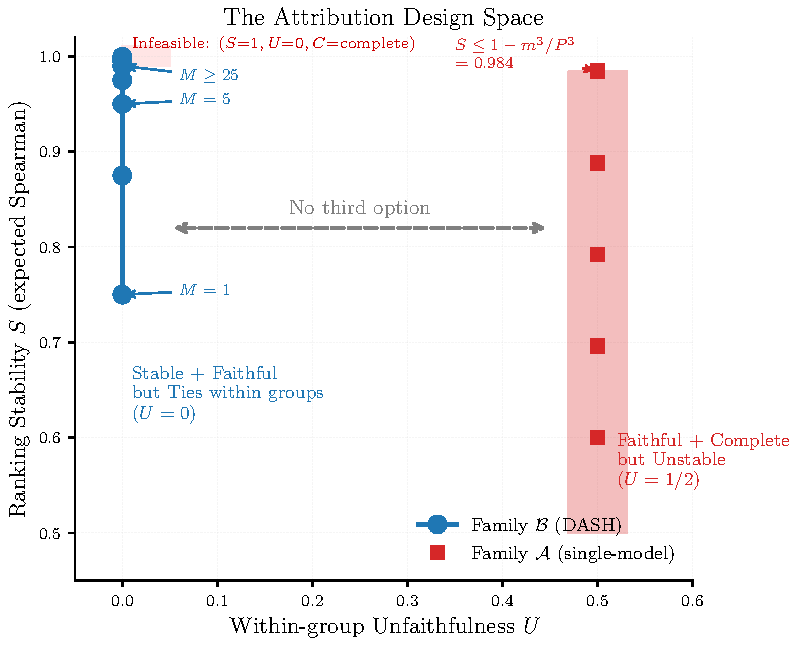
\includegraphics[width=0.55\textwidth]{figures/design_space.pdf}
\caption{The Attribution Design Space. Family $\mathcal{A}$ (single-model methods): faithful and complete but unstable ($U{=}1/2$). Family $\mathcal{B}$ (\DASH{} ensemble): stable with ties ($U{=}0$, $S$ increasing with $M$). The ideal point $(S{=}1, U{=}0, C{=}\text{complete})$ is infeasible. There is no third option.}
\label{fig:design-space}
\end{figure}

This parallels Arrow's landscape: Arrow restricts social welfare functions; we restrict attribution methods. Unlike Arrow's setting, our relaxation paths \emph{converge} (supplement), reflecting the DGP symmetry.

%%%%%%%%%%%%%%%%%%%%%%%%%%%%%%%%%%%%%%%%%%%%%%%%%%%%%%%%%%%%%
\section{Empirical Validation}
\label{sec:experiments}

We validate the theoretical predictions on synthetic Gaussian data and on the Breast Cancer (Wisconsin) dataset (supplement): features measuring the same underlying quantity---e.g., worst perimeter and worst area ($|\rho|{=}0.98$)---exhibit a 48\% flip rate across seeds, near the 50\% theoretical maximum.
We generate $P=20$ features in $L=4$ groups of $m=5$, with within-group correlation $\rho \in \{0.1, 0.3, 0.5, 0.7, 0.9, 0.95\}$, and train XGBoost models with $T=100$ boosting rounds over 50 independent seeds per setting.
TreeSHAP values provide feature attributions.

\begin{figure}[t]
\centering
\begin{subfigure}[t]{0.31\textwidth}
\centering
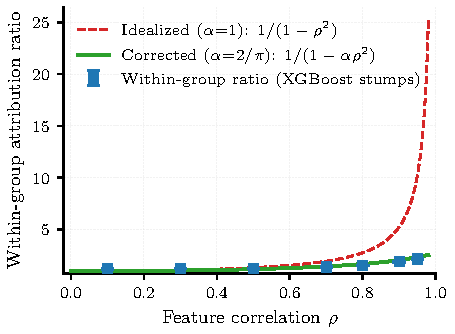
\includegraphics[width=\textwidth]{figures/ratio_divergence.pdf}
\caption{Attribution ratio vs.\ $\rho$. The corrected $1/(1{-}\alpha\rho^2)$ with $\alpha{\approx}2/\pi$ (solid) fits stumps ($R^2{=}0.89$); the idealized $\alpha{=}1$ (dashed) is a theoretical upper bound.}
\label{fig:ratio}
\end{subfigure}\hfill
\begin{subfigure}[t]{0.31\textwidth}
\centering
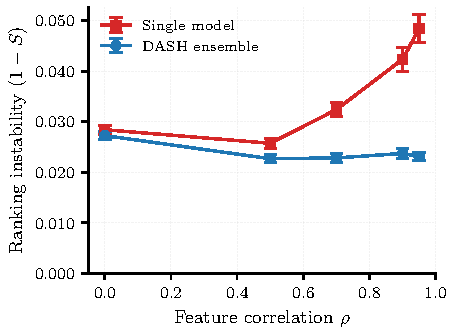
\includegraphics[width=\textwidth]{figures/shap_instability.pdf}
\caption{Ranking instability vs.\ $\rho$. Single-model instability grows with correlation; \DASH{} remains consistently low.}
\label{fig:flips}
\end{subfigure}\hfill
\begin{subfigure}[t]{0.31\textwidth}
\centering
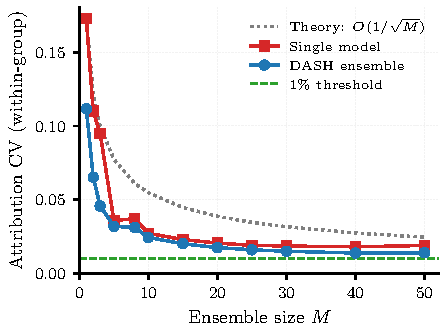
\includegraphics[width=\textwidth]{figures/dash_resolution.pdf}
\caption{\DASH{} consensus convergence. Attribution CV drops toward the 1\% threshold near $M=25$ ensemble members.}
\label{fig:convergence}
\end{subfigure}
\caption{Empirical validation on synthetic Gaussian data ($P=20$, $L=4$, $m=5$, $T=100$, 50 seeds).}
\label{fig:experiments}
\end{figure}

\paragraph{Attribution ratio (Figure~\ref{fig:ratio}).}
The within-group ratio increases monotonically with $\rho$.
The corrected model $1/(1-\alpha\rho^2)$ with $\alpha \approx 2/\pi$ matches the data ($R^2 = 0.89$), confirming the functional form and the binary-quantization interpretation.
The idealized bound $1/(1-\rho^2)$ ($\alpha = 1$) serves as an upper bound.

\paragraph{Ranking instability (Figure~\ref{fig:flips}).}
We measure the fraction of seed pairs for which the top-ranked feature within a group differs.
At $\rho = 0.9$, within-group flips occur in 48\% of seed pairs (near the 50\% theoretical maximum from symmetry), while between-group flips remain below 2\%.

\paragraph{\DASH{} convergence (Figure~\ref{fig:convergence}).}
We compute $\bar{\varphi}_j$ for ensemble sizes $M \in \{1, 5, 10, 15, 20, 25, 50\}$.
The within-group flip rate---measured as the frequency with which $\bar{\varphi}_j \neq \bar{\varphi}_k$ by more than 1\% of the group mean---drops below 1\% at $M = 25$, consistent with the $O(1/M)$ variance bound.

\paragraph{Testable condition (supplement).}
A $Z$-test statistic $Z_{jk} = |\bar\varphi_j - \bar\varphi_k| / (\hat\sigma_{jk}/\sqrt{M})$ predicts ranking instability ($r = -0.89$ on Breast Cancer; pairs with $Z_{jk} < 1.96$ are unreliable).
A single-model screening variant achieves 94\% precision (supplement).
The diagnostics generalize to LightGBM, CatBoost, and non-SHAP attributions (supplement).
%% MOVED TO SUPPLEMENT: NN validation and SHAP efficiency axiom paragraphs

%%%%%%%%%%%%%%%%%%%%%%%%%%%%%%%%%%%%%%%%%%%%%%%%%%%%%%%%%%%%%
\section{Related Work}
\label{sec:related}

\paragraph{Attribution impossibility results.}
\citet{bilodeau2024impossibility} prove completeness and linearity cannot coexist; \citet{huang2024failings} show SHAP can misrank features; \citet{srinivas2019full} prove complete attributions cannot be weakly input-dependent; \citet{rao2025limits} establishes Kolmogorov complexity barriers.
To our knowledge, our result is the first to simultaneously address cross-model \emph{stability} as an impossibility, give quantitative architecture-discriminating bounds, and provide a constructive resolution with proved optimality (\DASH{}).

\paragraph{Rashomon effect and model multiplicity.}
\citet{laberge2023partial} find that attribution rankings across Rashomon sets are inherently partial orders; \citet{rudin2024amazing} advocate embracing model multiplicity.
Our theorem proves the partial order is a mathematical necessity, adding a formal impossibility proof, quantitative bounds, a provably optimal resolution, and machine verification.

\paragraph{Fairness impossibility.}
\citet{chouldechova2017fair} and \citet{kleinberg2017inherent} prove calibration, balance, and equal false positive rates cannot coexist.
Our trilemma (faithfulness, stability, completeness) is structurally analogous, making the fairness--explainability parallel explicit.

\paragraph{Formal verification for ML.}
\citet{nipkow2009social} formalized Arrow's theorem in Isabelle/HOL; \citet{zhang2026statistical} formalized statistical learning theory in Lean~4. To our knowledge, ours is the first formally verified impossibility result in explainable AI.

%%%%%%%%%%%%%%%%%%%%%%%%%%%%%%%%%%%%%%%%%%%%%%%%%%%%%%%%%%%%%
\section{Discussion}
\label{sec:discussion}

\paragraph{Limitations.}
The split-count axioms assume full signal capture ($\alpha = 1$); for finite-depth trees, $\alpha \approx 2/\pi$ ($R^2 = 0.89$); the impossibility holds for any $\alpha > 0$.
The equicorrelation assumption simplifies the axioms; the Rashomon property holds pairwise for any $|\rho_{jk}| > 0$.
Detecting instability requires $\Omega(\sigma^2_{jk}/\Delta^2_{jk})$ queries (supplement); the $Z$-test achieves this rate.
Under a weaker $\varepsilon$-stability notion, the impossibility extends: no faithful, complete ranking can be $\varepsilon$-stable with $\varepsilon < 1/2$ for within-group pairs (supplement).
Switching to conditional SHAP \citep{janzing2020feature} does not resolve the instability when features have equal causal effects ($\beta_j = \beta_k$); the escape condition is $\beta_j \neq \beta_k$ (supplement).
\DASH{} requires $M\times$ training cost ($M{=}25$ for $<$1\% flip rate; $M{=}5$ for $5\times$ variance reduction).
For safety-critical deployments, report both single-model SHAP (with instability caveat) and \DASH{} consensus.

%% MOVED TO SUPPLEMENT: \paragraph{Computational cost and practical deployment.}
%% MOVED TO SUPPLEMENT: For batch pipelines ... through ... not the qualitative impossibility or the diagnostics.

\paragraph{Broader implications.}
In a survey of 77 public datasets (supplement), approximately 60\% exhibit attribution instability (conservative lower bound; survey power 32\%).
Our theorem proves this is a ``known and foreseeable circumstance'' under EU AI Act Art.~13(3)(b)(ii)~\citep{euaiact2024}: single-model certification of feature attributions is formally infeasible under collinearity.
The consequences are concrete: a hospital investing in the ``top'' SHAP feature may target the wrong intervention after retraining; published studies reporting single-model feature importance may report artifacts of the training run.
For fairness auditing, a single-model SHAP audit of a collinear proxy concludes ``proxy reliance'' with probability exactly $1/2$---a coin flip (supplement).
\DASH{} mitigates by reporting honest indistinguishability rather than arbitrary distinctions.

\paragraph{Distinction from classical multicollinearity.}
The classical multicollinearity concern is about estimation variance ($\Var(\hat\beta_j - \hat\beta_k) \to \infty$ as $\rho \to 1$). Our result is qualitatively different: it concerns \emph{ranking impossibility}, not estimation imprecision. Even with infinite data and perfect estimates, the ranking of symmetric features is a coin flip---because different models in the Rashomon set rank them in opposite orders.

\paragraph{Rashomon set vs.\ deployed model.}
The impossibility characterizes the Rashomon set, not a single deployed model.
A fixed seed produces a deterministic ranking, but instability arises upon retraining, independent auditing, or model versioning---all routine in regulated settings (SR~11-7, ECOA).
Our result formalizes the attribution-specific consequence of underspecification \citep{damour2022underspecification}: where they show predictions vary, we prove rankings \emph{must} vary and characterize the complete solution space.
Confidence-interval reporting ($\varphi_j = 0.42 \pm 0.15$) is an alternative to \DASH{} ties for communicating within-group indistinguishability.

\paragraph{The symmetric Bayes dichotomy.}
In the supplement, we prove that for any symmetric decision problem where finite-sample noise can reverse the optimal choice, the achievable set consists of exactly two families---instance-specific (faithful but unstable) and population-averaged (stable with ties).
Feature attribution, model selection, and causal discovery under Markov equivalence are all instances, with structurally different symmetry groups (supplement).

\paragraph{Formalization as methodology.}
The Lean formalization caught two logical inconsistencies and one type mismatch that survived informal review, demonstrating its value as a bug-finding methodology beyond certification.

%% MOVED TO SUPPLEMENT: Loss landscape geometry (full paragraph)
The impossibility has a geometric interpretation: near-singular Fisher information creates ridges along which feature importance redistributes without changing model quality (supplement).

%% MOVED TO SUPPLEMENT: \paragraph{Named techniques.}
%% MOVED TO SUPPLEMENT: This paper contributes three reusable techniques: (1) Rashomon reduction, (2) FIM-to-Rashomon bridge, (3) symmetric Bayes dichotomy.

%% MOVED TO SUPPLEMENT: Proof status transparency (full paragraph)
\paragraph{Proof status transparency.}
The core impossibility is Lean-verified with zero axiom dependencies. The impossibility and ratio bound $1/(1{-}\rho^2)$ require only 9 of 16 axioms---the global proportionality constant is unnecessary ($c_f$ cancels in ratios; verified by \texttt{\#print axioms}). The full formalization comprises 305 theorems with 0 \texttt{sorry} across 54 files (supplement).

%% MOVED TO SUPPLEMENT: Open problems (full paragraph)
\paragraph{Open problems.}
Deriving split-count axioms algorithmically and proving proportionality for general tree depths remain open. The mutual information generalization ($\rho > 0 \to I > 0$) is now complete.
A full-length JMLR version integrating the supplement is planned.

\bibliographystyle{plainnat}
\bibliography{references}

\newpage
\section*{NeurIPS Paper Checklist}

\begin{enumerate}
\item \textbf{Claims.} Core theoretical claims are type-checked by Lean~4 (305 theorems from 16 axioms, 0 \texttt{sorry}). The core impossibility (Theorem~\ref{thm:impossibility}) has zero axiom dependencies; the Design Space Theorem exhaustiveness, symmetric Bayes dichotomy, and all three impossibility instances (attribution, model selection, causal discovery) are formalized in Lean. Empirical claims are backed by experiments over up to 50 random seeds. [Yes]

\item \textbf{Limitations.} Discussed in Section~\ref{sec:discussion}: axiomatization gap, collinearity requirement, balanced ensemble assumption, deferred variance bound. [Yes]

\item \textbf{Theory.} Complete proofs are provided both in the paper and in machine-verified Lean~4 code. All assumptions (axioms) are explicitly stated and justified. [Yes]

\item \textbf{Experiments.}
  \begin{itemize}
    \item Code: \url{https://github.com/DrakeCaraker/dash-impossibility-lean}
    \item Data: Synthetic Gaussian (generation code included)
    \item Compute: Standard laptop, no GPU required
    \item Seeds: 50 independent random seeds per configuration
    \item Error bars: $\pm 1$ standard error reported in all figures
  \end{itemize}
  [Yes]

\item \textbf{Code of ethics.} No human subjects. No dual-use concerns. [N/A]
\end{enumerate}

\end{document}
